\documentclass[twocolumn,prb,aps,floatfix,superscriptaddress]{revtex4-1}

\usepackage{bm}%bold math
\usepackage{graphicx}
\usepackage{amsmath}
\usepackage{amssymb}
\usepackage{setspace}
\usepackage{epstopdf}
\usepackage{scalerel}
\epstopdfsetup{update} % only regenerate pdf files when eps file is newer
\linespread{1}
\usepackage[export]{adjustbox}

%\newcommand*\bplqt{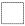
\includegraphics[height=1.6ex] {Symbols/blank_plqt}}
%\newcommand*\bhrzmv{\includegraphics[height=1.6ex]{Symbols/blank_hrzmv}}
%\newcommand*\bdiag{\includegraphics[height=1.6ex] {Symbols/blank_diag}}
%\newcommand*\bstr{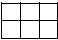
\includegraphics[height=1.6ex] {Symbols/blank_str}}

\newcommand{\figref}[1]{Fig. \ref{#1}}
\newcommand{\secref}[1]{Sec. \ref{#1}}

\newcommand*{\hprs}{%
  \text{% change size in subscripts or superscripts
    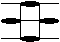
\includegraphics[
      height=1.2ex,% adjust to suit
      valign=M,% center vertically
      raise=\fontdimen22\textfont2,% but raise it to the formula axis
    ]{Symbols/hrzprestar} }
}
\newcommand*{\hspr}{%
  \text{% change size in subscripts or superscripts
    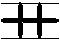
\includegraphics[
      height=1.2ex,% adjust to suit
      valign=M,% center vertically
      raise=\fontdimen22\textfont2,% but raise it to the formula axis
    ]{Symbols/hrzstarpair} }
}

\newcommand*{\bplqt}{%
  \text{% change size in subscripts or superscripts
    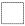
\includegraphics[
      height=1.2ex,% adjust to suit
      valign=M,% center vertically
      raise=\fontdimen22\textfont2,% but raise it to the formula axis
    ]{Symbols/blank_plqt} }
}
\newcommand*{\bhrzmv}{%
  \text{% change size in subscripts or superscripts
    \includegraphics[
      height=1.2ex,% adjust to suit
      valign=M,% center vertically
      raise=\fontdimen22\textfont2,% but raise it to the formula axis
    ]{Symbols/blank_hrzmv} }
}
\newcommand*{\bdiag}{%
  \text{% change size in subscripts or superscripts
    \includegraphics[
      height=1.2ex,% adjust to suit
      valign=M,% center vertically
      raise=\fontdimen22\textfont2,% but raise it to the formula axis
    ]{Symbols/blank_diag} }
}
\newcommand*{\bstr}{%
  \text{% change size in subscripts or superscripts
    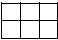
\includegraphics[
      height=1.2ex,% adjust to suit
      valign=M,% center vertically
      raise=\fontdimen22\textfont2,% but raise it to the formula axis
    ]{Symbols/blank_str} }
}
\newcommand*{\vvemptylink}{%
  \text{% change size in subscripts or superscripts
    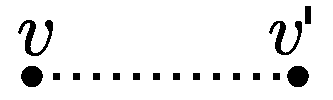
\includegraphics[
      height=1.8ex,% adjust to suit
      valign=M,% center vertically
      raise=\fontdimen22\textfont2,% but raise it to the formula axis
    ]{Symbols/string_net_link_sym0} }
}
\newcommand*{\emptylink}{%
  \text{% change size in subscripts or superscripts
    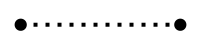
\includegraphics[
      height=1.5ex,% adjust to suit
      valign=M,% center vertically
      raise=\fontdimen22\textfont2,% but raise it to the formula axis
    ]{Symbols/string_net_link_sym1} }
}
\newcommand*{\rightarrowlink}{%
  \text{% change size in subscripts or superscripts
    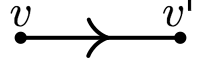
\includegraphics[
      height=1.5ex,% adjust to suit
      valign=M,% center vertically
      raise=\fontdimen22\textfont2,% but raise it to the formula axis
    ]{Symbols/string_net_link_sym2} }
}
\newcommand*{\leftarrowlink}{%
  \text{% change size in subscripts or superscripts
    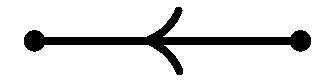
\includegraphics[
      height=1.5ex,% adjust to suit
      valign=M,% center vertically
      raise=\fontdimen22\textfont2,% but raise it to the formula axis
    ]{Symbols/string_net_link_sym3} }
}
\newcommand*{\twointwoout}{%
  \text{% change size in subscripts or superscripts
    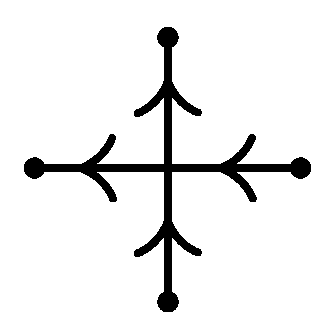
\includegraphics[
      height=1.5ex,% adjust to suit
      valign=M,% center vertically
      raise=\fontdimen22\textfont2,% but raise it to the formula axis
    ]{Symbols/two_in_two_out} }
}
\newcommand*{\oneinoneout}{%
  \text{% change size in subscripts or superscripts
    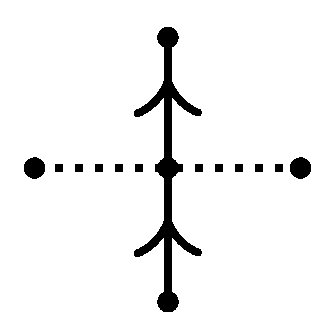
\includegraphics[
      height=1.5ex,% adjust to suit
      valign=M,% center vertically
      raise=\fontdimen22\textfont2,% but raise it to the formula axis
    ]{Symbols/one_in_one_out} }
}
\newcommand*{\threeinzeroout}{%
  \text{% change size in subscripts or superscripts
    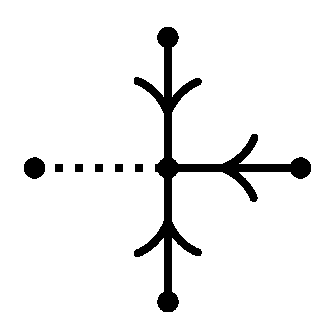
\includegraphics[
      height=1.5ex,% adjust to suit
      valign=M,% center vertically
      raise=\fontdimen22\textfont2,% but raise it to the formula axis
    ]{Symbols/three_in_zero_out} }
}
\newcommand*{\threeoutzeroin}{%
  \text{% change size in subscripts or superscripts
    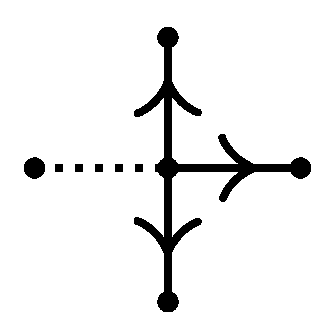
\includegraphics[
      height=1.5ex,% adjust to suit
      valign=M,% center vertically
      raise=\fontdimen22\textfont2,% but raise it to the formula axis
    ]{Symbols/three_out_zero_in} }
}
\newcommand*{\zerooutzeroin}{%
  \text{% change size in subscripts or superscripts
    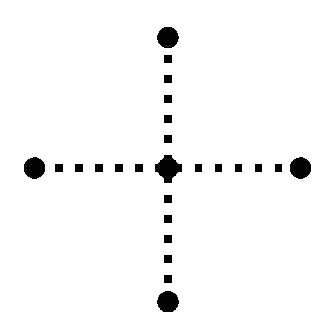
\includegraphics[
      height=1.5ex,% adjust to suit
      valign=M,% center vertically
      raise=\fontdimen22\textfont2,% but raise it to the formula axis
    ]{Symbols/zero_out_zero_in} }
}
\newcommand*{\hrzplqt}{%
  \text{% change size in subscripts or superscripts
    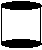
\includegraphics[
      height=1.5ex,% adjust to suit
      valign=M,% center vertically
      raise=\fontdimen22\textfont2,% but raise it to the formula axis
    ]{Symbols/hrzplqt.pdf} }
}
\newcommand*{\vrtplqt}{%
  \text{% change size in subscripts or superscripts
    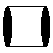
\includegraphics[
      height=1.5ex,% adjust to suit
      valign=M,% center vertically
      raise=\fontdimen22\textfont2,% but raise it to the formula axis
    ]{Symbols/vrtplqt.pdf} }
}

%%%%%%%%%%%%%%%%%%%%%%%%%%%%%%%%%%%%%%%%%%%%%%%%%%%%%%%%%%%%%%%%%%%%%%%%%%%%%%%%%%%%%%%%%%%%%%%
\begin{document}

\title{Topological order in the quantum dimer-pentamer model}

\author{Owen Myers}
\email{omyers@uvm.edu}
\affiliation{Department of Physics, University of Vermont, Burlington, VT 05405, USA}

\author{C. M. Herdman}
\affiliation{Institute for Quantum Computing, University of Waterloo, Ontario, N2L 3G1, Canada}
\affiliation{Department of Physics \& Astronomy, University of Waterloo, Ontario, N2L 3G1, Canada}
\affiliation{Department of Chemistry,  University of Waterloo, Ontario, N2L 3G1, Canada}

\begin{abstract}
We study the ground state of the quantum dimer-pentamer model (QDPM) on the square lattice. This model is a generalization of the square lattice quantum dimer model (QDM) as its configuration space comprises fully-packed hard-core dimer coverings as well as configurations containing pentamers, where four dimers touch a vertex. Thus in the QDPM, the fully-packed, hard-core constraint of the QDM is relaxed such that the local dimer number at each vertex is fixed modulo 3; correspondingly, the local $U(1)$ gauge symmetry of the QDM Hilbert space is reduced to a local $Z_3$ gauge symmetry in the QDPM. We construct a local Hamiltonian for which the Rokhsar-Kivelson (RK) state (the equal superposition of all configurations in a topological sector) is the exact ground state and has a 9-fold topological degeneracy on the torus. Using Monte Carlo calculations, we find no spontaneous symmetry breaking in the RK wavefunction and that its dimer-dimer correlation function decays exponentially. Additionally, we discuss the possibility of $Z_3$ topological order in the ground state of the QDPM.
\end{abstract}

\maketitle

%%%%%%%%%%%%%%%%%%%%%%%%%%%%%%%%%%%%%%%%%%%%%%%%%%%%%%%%%%%%%%%%%%%%%%%%%%%%%%%%%%%%%%%%%%%%%%%
%%%%%%%%%%%%%%%%%%%%%%%%%%%%%%%%%%%%%%%%%%%%%%%%%%%%%%%%%%%%%%%%%%%%%%%%%%%%%%%%%%%%%%%%%%%%%%%
\section{Introduction}

Over the last several decades, experimental and theoretical work has demonstrated that strongly interacting quantum many-body systems support exotic quantum phases phases of matter not described by the Landau symmetry breaking paradigm. One class of such quantum phases of matter are topologically ordered quantum liquids~\cite{Wen1990}, first realized experimentally via the fractional quantum Hall effect~\cite{FQHE????}. Despite the absence of conventional symmetry breaking and a local order parameter, topological quantum liquids possess a non-trivial quantum order that distinguishes them from trivial liquid phases~\cite{Nayak2008}. Although not detectable by local operators, topological order arises due to a non-local entanglement structure that leaves a signatures in the bipartite entanglement entropy~\cite{Levin2006a,Kitaev2006b}. Such topological phases provide the basis for a proposal for fault-tolerant quantum information processing~\cite{Freedman2001,Kitaev2003}.

Because of the exotic nature of topological phases and their potential use for quantum information processing, there is great interest in the development of theoretical models which display these phases. Such models offer the possibility of furthering the understanding of these phases as well as providing possibly candidate experimental systems in which to constructively engineer topological order~\cite{Duan2003,Jaksch2005,Lewenstein2007,Jiang2008d,Weimer2010a,Herdman2010c,Martinis2015}. A variety of exactly soluble lattice models are known to support ground states with topological order that ranges from the simplest variety, so-called $Z_2$ topological order~\cite{Kitaev2003,Wen2003}, to those with non-Abelian anyonic excitations~\cite{Levin2005a,Kitaev2006a}. These exactly soluble models generally involve complex many-body interactions, and thus it is desirable to find simpler models supporting topological order that are closer to what is accessible experimentally.

Among the simplest class of models displaying topological quantum liquid phases are those with local geometric constraints; the frustration inherent in these constraints inhibits the formation of symmetry breaking local order and given sufficient dynamics, such models may have symmetric liquid ground states. The simplest such geometrically constrained model is the quantum dimer model (QDM) describing dimer degrees of freedom living on the links of a lattice~\cite{Rokhsar1988,Moessner2008}; the hard-core, fully-packed QDM has a local constraint that requires exactly one dimer touching each vertex.

\begin{figure}[b!]
    \centering
    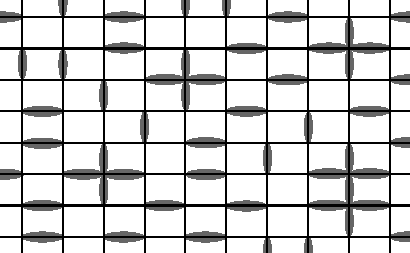
\includegraphics[width=0.5\columnwidth]{QDPM_ex_config.pdf}
    \caption{Example of an allowed configuration in the quantum dimer-pentamer model.}
    \label{fig:QDPMex}
\end{figure}

While on non-bipartite lattices, the QDM posses a topologically ordered ground state~\cite{Moessner2001a,Fendley2002}, on the square lattice there is only a liquid ground state at an isolated critical quantum point~\cite{Leung1996,Syljuasen2006}. If the hard-core constraint of the QDM is relaxed to a parity constraint such that each vertex much have an even (odd) number of dimers touching each vertex, the simplest non-trivial dynamics lead to the (odd) toric code which has a $Z_2$ topologically ordered ground state~\cite{Kitaev2003,Wen2003}. 

The existence of topologically ordered ground states in dimer-based models is intimately related to the local constraint which imposes a local gauge symmetry in the low energy Hilbert space; the topological order that arises is directly related to a discrete gauge theory with the appropriate local gauge constraint~\cite{Moessner2001}.

Given that these models with dimer degrees of freedom and local constraints posses the simplest non-trivial local (Ising) Hilbert space at each link, they provide a (possibly) simpler route to engineering exotic phases; the local constraints constraint can often be enforced by a local potential energy penalty and the required dynamics are generally expected to arise at the lowest order non-trivial order in perturbation theory. Previous work as demonstrated that GQDM on the square lattice support gapped $Z_2$ topologically ordered phases as well as gapless quantum critical points. On non-bipartite lattices GQDM supported $Z_2$ topological order~\cite{Moessner2001a,Misguich2002} as well as doubled-semion phases~\cite{Qi2014,Buerschaper2014a}. A full characterization of all exotic phases that can exist within this framework is thus desirable.

In this work we extend this paradigm to a new GQDM on the square lattice, what we term the quantum dimer-pentamer model (QDPM). In the QDPM, the local constraint is relaxed from that of the QDM to require that either $1$ or $4$ dimers to touching each vertex, as shown in figure \figref{fig:QDPMex}. Correspondingly, the QDPM extends the Hilbert space of the QDM to include both fully-packed hard-core dimer configurations, as well as those pentamers, four dimers touch a vertex. To give the system dynamics, the Hamiltonian includes terms that incorporate the simplest non-trivial dynamics that don't violate the local constraint.

We present a numerical study of the ground state of the QDPM at an exactly soluble point and demonstrate the the soluble point represents a gapped, disordered quantum liquid phase.  Using Monte Carlo calculations, we explicitly demonstrate the absence of symmetry breaking order and the exponential decay of correlation functions; by computing imaginary-time correlation functions, we find that the RK point is gapped in the thermodynamic limit. By construction the QDPM has an exact local $Z_3$ symmetry and conserves a $Z_3$ topological winding number. Thus the QDPM has a 9-fold topological degeneracy on the torus. Thus we argue that the ground state of the QDPM posses $Z_3$ topological order.

This this paper is organized as follows. In \secref{sec:Background} we provide relevant background for the QDM and related models. In \secref{sec:QDPM} we present the details of the QPDM. \secref{sec:MC} provides the results of a Monte Carlo study of the ground state of the QDPM at its exactly soluble point.


%%%%%%%%%%%%%%%%%%%%%%%%%%%%%%%%%%%%%%%%%%%%%%%%%%%%%%%%%%%%%%%%%%%%%%%%%%%%%%%%%%%%%%%%%%%%%%%
\section{Background}
\label{sec:Background}

\subsection{Generalized quantum dimer models}
\label{sec:GQDM}

\begin{figure}[htpb]
    \centering
    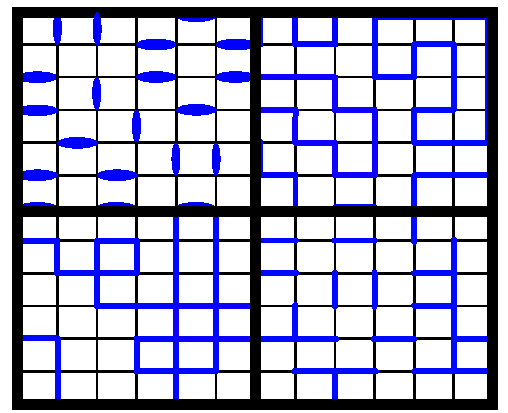
\includegraphics[width=0.8\linewidth]{example_local_constraints.pdf}
    \caption{Clockwise from the upper left panel we show an example of a QDM with constraints: one
    dimer, two dimers, an even number of dimers, and and odd number of dimers touching each vertex.}
    \label{fig:example_local_constraints}
\end{figure}

Here we will provide background about generalized quantum dimer models on the square lattice. We consider systems with Ising-like dimer degrees of freedom on each link, such that each link has either $0$ or $1$ dimers. The Hilbert space consists of configurations of dimers on the square lattice that satisfy a local constraint at each vertex; the simplest constraint is that of the hard-core fully-packed QDM where a single dimer must touch each vertex. We write this constraint as $n_v = 1$, where $n_v$ is the number of dimers that touch a vertex. We can distinguish between number constraints of the form $n_v = n_0$ and parity constraints of the form $n_v \mod 2 = 0,1$. The unique, non-trivial constraints of this form are the number constraints $n_v=1,2$ and the parity constraints $n_v\mod2 =0,1$ and  $n_v\mod2 =1$ (see \figref{fig:GQDMexamples}).

The presence of such local constraints implies all physical states in the Hilbert space are invariant under local gauge transformations at each vertex, $G_v$. 

The Hamiltonian of a GQDM is of the form
\begin{equation}
H_{\rm{GQDM}} = -t \hat{T} + v \hat{V}
\end{equation}
where $\hat{T}$ is an off-diagonal kinetic term that preserves the constraint, $\hat{V}$ is a local potential energy term, and $v$ and $t$ parametrize the strength of each term. We will take the kinetic term $\hat{T}$ to be the dynamics which preserved the constraint; for example in the QDM $\hat{T}$ is the sum of all possible ``plaquette" flip terms acting on plaquettes with parallel dimers.
\begin{equation}
    \label{}
    \hat{T} = \sum_{\bplqt} 
            \left|
                \vrtplqt
            \right\rangle
            \left\langle
                \hrzplqt
            \right|
            +
            \mathrm{h.c.}
\end{equation}

    Now we will introduce the toric code on the square lattice in some detail to sever as a point of reference and
    comparison for the following discussion of the $Z_3$ case. The toric code Hamiltonian is given by
    %
    \begin{equation}
        H_t = -J_e\sum_v A_v - J_m\sum_p B_p
        \label{eqn:toric_code_ham}
    \end{equation}
    %
    where the operator $A_v$ acts on the vertex $v$ and the sum over $v$ is the sum over all vertices. 
    The operator $B_p$ acts on a plaquette $p$ and the sum over $p$ is the sum over all
    plaquettes. In the $Z_2$ toric code, Ising degrees of freedom live on the links of the
    lattice. Explicitly the operators $A_v$ and $B_p$ can be expressed as
    %
    \begin{equation}
        A_v = \prod_{i\in v} \sigma^x_i
        ,
    \end{equation}
    %
    and
    \begin{equation}
        B_p = \prod_{i\in p} \sigma^z_i
        .
    \end{equation}
    %
    The products are over the links adjacent to vertex $v$ and on the edges of plaquette $p$ for
    $A_v$ and $B_p$ respectively. Since all $A_v$ operators commute with each other, all
    $B_p$ operators commute with each other and $A_v$ commutes with $B_p$ even if they share
    links (commute because they
    can only share an even number of links) then the Hamiltonian can be solved term by term.

    Without a rigorous solution it is possible to guess at the form of the Toric code
    ground state wave function. The first term in \ref{eqn:toric_code_ham} is maximized ($H_t$
    minimized) when an even number of links touching a vertex are spin up or down in the
    $\sigma^z$ basis. By coloring the links of all down spins the groundstate will
    contain closed loops. The second term in \ref{eqn:toric_code_ham} is maximized for a
    superposition of loops since $B_p$ flips the spins around a plaquette $p$. The ground state
    wave function is then a superposition of all possible closed loop configurations. 
    %Since $B_p$ is a local operator
    %though the alowed loop configurations are determined by how the sytem in initilized.
    
    NEED HERE Some stuff about plaquette flux ?? -> $B_p | \Psi \rangle = | \Psi \rangle$ -> only true if
    grnd state as no vortices

    NEED HERE String operators. The electric and magnetic string operators are respectively
    \begin{equation}
        S^e_{\Gamma} = \prod_{i\in\Gamma_e} \sigma^x_i
        ,
    \end{equation}
    \begin{equation}
        S^m_{\Gamma} = \prod_{i\in\Gamma_m} \sigma^z_i
        ,
    \end{equation}
    where the path is denoted by $\Gamma$. The path of the electric string operator is along the
    links of the lattice and if this path is not closed then the operator
    creates a pair of excitations. These excitations are defects in the system 
    that can be thought of as electric charges that live at the
    end of the unclosed string. Each of these electric defects has an energy costs of $2J_e$. 
    The path of the magnetic string operator runs perpendicular to the links
    and starts and ends on the dual lattice. An unclosed magnetic path results in two magnetic
    excitations on the at the ends of the magnetic string each costing $2J_m$ each. 

    Using a nontrivial path (genus of system $>0$) one can move between topological sectors using $S_e$ and determine
    the topological sector the system is in using $S_m$. On a torus, acting with $S_e$ along a
    path that encloses either the major or minor axis of the torus changes the topological sector.
    In general there are $4^g$ topological sectors where $g$ is the
    genus of the system. For a torus then there are four topological sectors. If These can be
    measuerd using the $S_m$ operator on a ...




    \subsection{$Z_3$ Toric Code}
        We can represent the $Z_3$ algebra through the following expressions
        %
        %Z_N
        %\begin{equation}
        %    E |n\rangle = n |n\rangle, ~ n=0,1,2,...,N-1
        %    \\
        %    e^{iA} |n\rangle = |n+1 \rangle, ~ n=0,1,2,...,N-2
        %    \\
        %    e^{iA} |N-1\rangle = |0\rangle
        %    %\label{eqn:}
        %\end{equation}
        %Z_3
        %
        \begin{equation}
            \begin{split}
            & E_l |n_l\rangle = n_l |n_l\rangle, ~ n_l=0,1,2
            \\
            & e^{iA_l} |n_l \rangle = |n_l+1 \rangle, ~ n_l =0,1
            \\ 
            & e^{iA_l} |2 \rangle = |0\rangle
            \end{split}
            ,
            %\label{eqn:}
        \end{equation}
        %
        where the operators $E_l$ and $A_l$ act on a given link $l$ and are analogous to the electric field and vector potential
        respectively. 
        By assigning orientations to the links between two vertices we can define 3 unique
        link ``values'' pictorially. 
        %
        \begin{itemize}
            \item $\vvemptylink$ 
            \item $\rightarrowlink$ 
            \item $\leftarrowlink$ 
        \end{itemize}
        % 
        In this way we can define $e^{iA_l}$ as the operator $Q$ which acts on the links in the
        following way
        \begin{equation}
            \begin{split}
                & Q^\dagger_{vv'}  | \vvemptylink \rangle = | \rightarrowlink \rangle
                ,
                \\
                & Q^\dagger_{vv'}  | \rightarrowlink \rangle = | \leftarrowlink \rangle
                ,
                \\
                & Q^\dagger_{vv'}  | \leftarrowlink \rangle = | \emptylink \rangle
                ,
            \end{split}
            %\label{eqn:}
        \end{equation}
        where the link is specified by the two vertices it connects and the operator
        $Q^\dagger_{vv'}$ acts in a direction from vertex $v$ to vertex $v'$. By changing the
        direction in which $Q$ operates we can express it in terms of its hermitian conjugate. 
        %
        \begin{equation}
            (Q^\dagger_{vv'})^\dagger = Q_{vv'}^\dagger
            .
            %\label{eqn:}
        \end{equation}

        The operator $E$ The operator $E_{vv'}$ can be defined in a similar way as
        %
        \begin{equation}
            \begin{split}
                & E^\dagger_{vv'}  | \vvemptylink \rangle = 0
                ,
                \\
                & E^\dagger_{vv'}  | \rightarrowlink \rangle = | \rightarrowlink \rangle
                ,
                \\
                & E^\dagger_{vv'}  | \leftarrowlink \rangle = 2| \leftarrowlink \rangle
                ,
            \end{split}
            %\label{eqn:}
        \end{equation}
        and with it we can define.
        %
        \begin{equation}
            P_{vv'}^\dagger \equiv e^{i2\pi E_{vv'}/3}
            .
            %\label{eqn:}
        \end{equation}
        %
        Now how $P_{vv'}^\dagger$ acts on the links: 
        %
        \begin{equation}
            \begin{split}
                & P^\dagger_{vv'}  | \vvemptylink \rangle = | \vvemptylink \rangle
                ,
                \\
                & P^\dagger_{vv'}  | \rightarrowlink \rangle = e^{i2\pi/3} | \rightarrowlink \rangle
                ,
                \\
                & P^\dagger_{vv'}  | \leftarrowlink \rangle = e^{-i2\pi/3} | \leftarrowlink \rangle
                .
            \end{split}
            %\label{eqn:}
        \end{equation}
        %

        The $Z_3$ toric code Hamiltonian can now be written in terms of the $P$ and $Q$ operators. The
        usual string net Hamiltonian is written as 
        \begin{equation}
            H = - J_e \sum_v A_v - J_m \sum_p B_p
            %\label{eqn:}
        \end{equation}
        where the sum over $v$ and the sum over $p$ are the sums over all vertices and plaquettes on
        the lattice respectively and 
        \begin{equation}
            A_v = \prod_{i\in v} P^\dagger_{vv_i}~,~ B_p \prod_{i\in p} Q^\dagger_{v_iv_{i+1}}
            .
            %\label{eqn:}
        \end{equation}
        The specific vertex and plaquette labeling scheme is shown in Fig.~\ref{fig:vertex_link_labels}.
        %
        \begin{figure}[htpb]
            \centering
            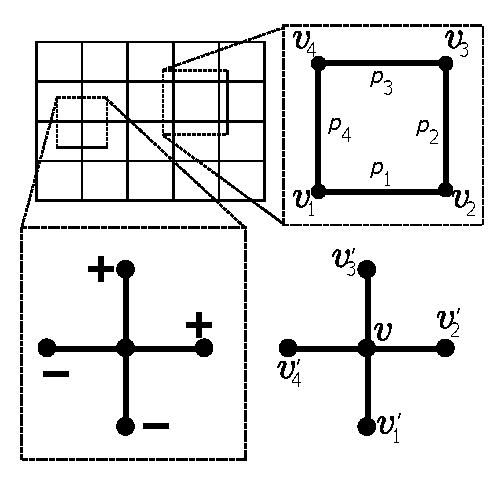
\includegraphics[width=0.8\linewidth]{vertex_link_gauge_def}
            \caption{Notation of vertex and plaquette labels}
            \label{fig:vertex_link_labels}
        \end{figure}
        %
        For the ground state of this Hamiltonian there is a local symmetry corresponding to the
        minimization of the first term. The model has an exactly local gauge symmetry that can be
        expressed as
        \begin{equation}
            G_v | \psi \rangle= | \psi \rangle
            %\label{eqn:}
        \end{equation}
        where $G_v$ = $A_v$.


        \subsubsection{Hamiltonian Gauge symmetry }


        \subsubsection{String operators}
            With the above notation we can write down the string operators. The electric string operator along
            the path $\Gamma_{v_b v_e}$ between the two vertices $v_0$ (beginning) and $v_N$ (end) is written
            %
            \begin{equation}
                S^e_{\Gamma} = \prod_{l=0}^{N-2} Q_{v_lv_{l+1}}^\dagger
                %\label{eqn:}
                ,
            \end{equation}
            %
            where $v_l \in \Gamma$ and $N$ is the number of vertices in $\Gamma$. We show an example of an
            electric string operator operation on an example configuration in Fig.~\ref{fig:example_elec_string}.
            %
            %
            \begin{figure}[htpb]
                \centering
                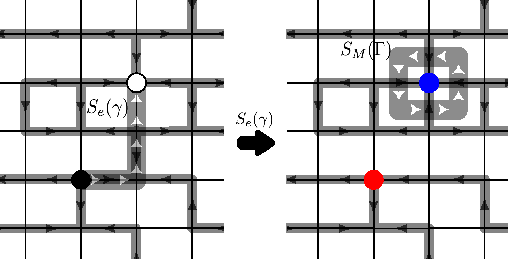
\includegraphics[width=0.8\linewidth]{example_elec_string.pdf}
                \caption{The grey line is the path $\Gamma$ on which the string operator acts. The operator acts
            in the direction from the vertex labeled in red to the one labeled in blue.}
                \label{fig:example_elec_string}
            \end{figure}
            %
            %
            The magnetic string operator can be written as
            \begin{equation}
                S^m_{\Gamma} = \prod_{l=0}^{N-1} Q_{v_{2l}v_{2l+1}}^\dagger
                %\label{eqn:}
            \end{equation}
            %
            where $v_l$ are the vertices adjacent to the links in $\Gamma$ and $N$ is the number of
            vertices
            on the \textit{left} side of the path when looking along the path from red to blue. 
            An example of this operator acting
            on a configuration is shown in Fig.~\ref{fig:example_mag_string} along with the vertex labeling
            scheme.
            %
            %
            \begin{figure}[htpb]
                \centering
                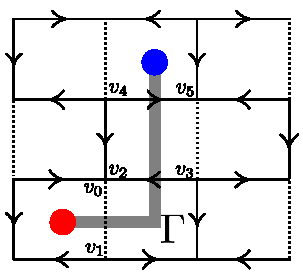
\includegraphics[width=0.8\linewidth]{example_mag_string.pdf}
                \caption{The grey line is the path $\Gamma$ on which the string operator acts. The magnetic
                    string operator acts in the 
                    direction from the plaquette labeled in red to the one labeled in blue.}
                \label{fig:example_mag_string}
            \end{figure}
            %
            The magnetic string operator acting on path $\Gamma$ in Fig.~\ref{fig:example_mag_string} is
            explicitly
            %
            \begin{multline}
                S^m_{\Gamma} (\mathrm{~Fig.~\ref{fig:example_mag_string}~config})
                = P_{v_0v_1}^\dagger P_{v_2v_3}^\dagger P_{v_4v_5}^\dagger
                \\
                = \exp{[0 - \frac{i2\pi}{3} + \frac{i2\pi}{3} ]} 
                = 1 (\mathrm{~Fig.~\ref{fig:example_mag_string}~config})
                .
            \end{multline}
            %

            An interesting property of the electric string string operators in the $Z_3$ toric code is
            that they produce two defects, one having positive charge and the other having negative
            charge. This is most easily see by looking at Fig.~\ref{fig:example_elec_string}. The
            configuration in Fig.~\ref{fig:example_elec_string}(a) obeys the local gauge symmetry and
            when the electric string operator acts on path $\Gamma$ it results in two defects at the
            end points of $\Gamma$. At the first $v_0$ (red) the local constraint is broken and
            $G_{v_0} = e^{i2\pi /3}$ as shown in Fig.~\ref{fig:example_elec_string}(b), whereas
            $G_{v_3} = e^{-i2\pi /3}$ which can be thought of as negative and positive gauge charges
            at $v_0$ and $v_3$ respectively.

            The magnetic excitations, or $Z_3$ visons live at the endpoints of a path created with the magnetic
            string operator. These visons can take three different values which can be changed by
            operating with the electric operator on a path that encircles one endpoint of the
            magnetic string path. 


        \subsubsection{properties of $Z_3$ string operators}

        \subsubsection{Winding Numbers}

            The ground state of the $Z_3$ toric code on the torus is nine-fold degenerate because of
            the nine different topological sectors in this topology. One can move between the
            topological sectors with a nontrivial closed electric string wraps around either
            the major axis or the minor axis of the torus. We will call the electric winding
            operator that acts around the major axis $W^e_y$ and around the minor axis $W^e_x$.
            A given topological sector can be distinguish 
            by acting around the minor and major axes with the magnetic string operator $W^m_y$ and
            $W^m_x$. All of the aforementioned winding operators commute with the Hamiltonian and
            therefore share the same eigenvalues. The operator $W^m_{x}$ ($W^m_{y}$) can 
            have three different values depending on how many electric strings enclose the minor
            (major) axis. Since there are three different
            possible values for each winding number around each axis there are nine distinct
            topological sectors.

            \begin{figure}[htpb]
                \centering
                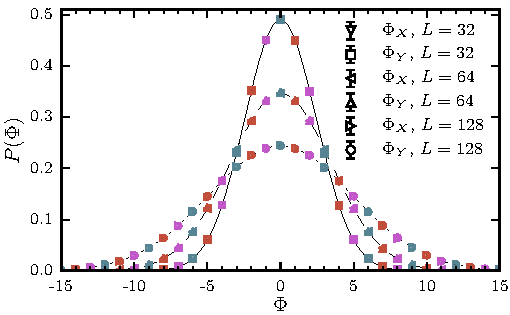
\includegraphics[width=0.8\linewidth]{u1_wind_qdpm.pdf}
                \caption{The $U(1)$ winding number as measured in the QDPM on a $8\times8$ lattice
                with a dimer to pentamer move fraction (need a name for this fraction HERE) of 0.5.}
                \label{fig:u1_wind_qdpm}
            \end{figure}


    \subsection{QDM on Square lattice}
        Here we will review the relevant
        properties and attributes of the QDM on the square lattice for which the Hamiltonian is.
        \begin{equation}
            \label{}
            H_{\mathrm{QDM}} = -t\sum_{\bplqt} 
                \left(
                    \left|
                        \vrtplqt
                    \right\rangle
                    \left\langle
                        \hrzplqt
                    \right|
                    +
                    \mathrm{h.c.}
                \right)
            - v\sum_{\bplqt}
                \left(
                    \left|
                        \vrtplqt
                    \right\rangle
                    \left\langle
                        \vrtplqt
                    \right|
                    +
                    \left|
                        \hrzplqt{}
                    \right\rangle
                    \left\langle
                        \hrzplqt
                    \right|
                \right)
                .
        \end{equation}
        This model can be defined in terms of a single parameter $t/v$ for which the wave function is
        known exactly at the Rokhsar and Kivelson (RK) point, the point where $t/v =1$. At the RK
        point the wave function is the equal weighted superposition over all dimer configurations.
        HERE



%%%%%%%%%%%%%%%%%%%%%%%%%%%%%%%%%%%%%%%%%%%%%%%%%%%%%%%%%%%%%%%%%%%%%%%%%%%%%%%%%%%%%%%%%%%%%%%
%%%%%%%%%%%%%%%%%%%%%%%%%%%%%%%%%%%%%%%%%%%%%%%%%%%%%%%%%%%%%%%%%%%%%%%%%%%%%%%%%%%%%%%%%%%%%%%
\section{The Quantum Dimer Pentamer Model}

    \subsection{Local $Z_3$ Gauge Symmetry}

        In the QDPM Ising degrees of freedom live on the links of the lattice.
        The operator $\hat{\sigma}^x_l$ acts on these links and has 
        eigenvalues $\sigma_l = \pm 1$, where $\sigma_l$ is the
        Ising variables of the $l^{\mathrm{th}}$ link on the lattice. The number operator for a give link is
        defined as $\hat{n}_l \equiv (1+\hat{\sigma}_x)/2$ and counts the number of dimers on link $l$.
        An exactly local gauge symmetry exists on the lattice due to the constraint that either one or
        four dimers touch any give vertex. In terms of $n_l$ we can define an operator that counts the
        number of dimers touching a given vertex $v$ as $n_v = \sum_{l\in v} n_l$. 
        
        the local gauge transformation $G_v$ acting on a give vertex $v$ for the quantum dimer model
        can be expressed as
        %
        \begin{equation}
            \label{}
            G_v=e^{i \alpha (n_v - n_0)}
        \end{equation}
        %
        where $n_0$ is the constrained number of dimers touching a vertex, $n_0=1$ in the QDM model,
        The operator $G_v$ then acts in such a
        way that only the physical states, states satisfying the local constraint 
        are invariant. For the QDM $G_v =
        e^{i\alpha (0)}$ and therefore $G_v$ leaves a physical state unchanged for any
        $\alpha$ making the local gauge symmetry $U(1)$. The local gauge transformation that leaves
        only configurations containing dimers and pentamers invariant is
        %
        \begin{equation}
            \label{eqn:gauge_trans}
            G_v = e^{i (\hat{n}_v -1) 2\pi/3}    
        \end{equation}
        %
        For the QDPM $\alpha$ is must be $2\pi/3$ due to the relaxed constraint of the QDM
        model that allows for pentamers. Relaxing the constraint of the QDM brings the local gauge
        symmetry from $U(1)$ to $Z(3)$.

    \subsection{QDPM Hamiltonian}

        We work specifically at the RK point at which the ground state wave function
        is an equal weighted superposition of fully packed dimer pentamer configurations
        %
        \begin{equation}
            \label{}
            \left| \Psi \right\rangle = \frac{1}{\sqrt{N}}\sum_{\{C\}} \left| C \right\rangle
            ,
        \end{equation}
        %
        where $\{C\}$ is the set of fully packed configurations. The Hilbert space can be defined
        using the gauge transformation in Eq.~\ref{eqn:gauge_trans} as all $\left| C \right\rangle$
        satisfying $G \left| C \right\rangle = \left| C \right\rangle$.

        The QDPM Hamiltonian
        \begin{equation}
            H_{\mathrm{QDPM}} = H_{\mathrm{QDM}} + \mathrm{pentamer\ terms}
        \end{equation}

        The pentamer terms in the Hamiltonian can be constructed with the dynamics shown in
        Fig.~\ref{fig:pentamer_moves}.  
        \begin{figure}[htpb]
            \centering
            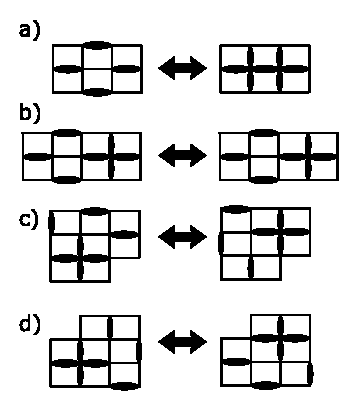
\includegraphics[width=0.8\linewidth]{pentamer_moves.pdf}
            \caption{a) Horizontal creation an annihilation, b) horizontal move, c) and d) are two
            different possible diagonal moves in the same direction.}
            \label{fig:pentamer_moves}
        \end{figure}
        Each of the  moves shown in Fig.~\ref{fig:pentamer_moves} can be
        rotated to produce the symmetry related counterpart (eg. vertical creation and annihilation). 
        As an example the creation and annihilation term in the Hamiltonian is
        \begin{multline}
        H_{\mathrm{pentamer\ creation}} = t_{\mathrm{create}}
            \sum_{\bstr}
            \left(
                \left|
                    \hprs
                \right\rangle
                \left\langle
                    \hspr
                \right|
                +
                \mathrm{h.c.}
            \right)
            \\
            - v_{\mathrm{create}}
            \sum_{\bstr}
                \left(
                    \left|
                        \hprs
                    \right\rangle
                    \left\langle
                        \hprs
                    \right|
                    +
                    \left|
                        \hspr
                    \right\rangle
                    \left\langle
                        \hspr
                    \right|
                \right)
        \end{multline}
        where the factors $t_{\mathrm{create}}$ and $v_{\mathrm{create}}$ are the coefficients of
        the pentamer pair creation and annihilation respectively. At the RK point
        $t/v=1$ for each all the pentamer terms. 
        Writing the kinetic and potential energy terms as done above for all the dynamics shown in
        Fig.~\ref{fig:pentamer_moves} and all of their symmetry related counterparts comprise the
        the pentamer terms of the Hamiltonian. 

    \subsection{Winding operators}

        In the QDPM there is a conserved winding operator in a given topological sector
        \begin{equation}
            W_{x,y} = (N_A - N_B)\mod{3} = n
            .
        \end{equation}
        For $W_y$ ($W_x$), $N_A$ is the number of dimers crossed on a vertical (horizontal) cut and
        $n=0$, $1$, or $2$ depending on the topological sector. The winding operator commutes with
        the Hamiltonian and therefore share the same eigenvalues. Since there are three winding numbers in
        each direction then the ground state is ninefold degenerate.

%%%%%%%%%%%%%%%%%%%%%%%%%%%%%%%%%%%%%%%%%%%%%%%%%%%%%%%%%%%%%%%%%%%%%%%%%%%%%%%%%%%%%%%%%%%%%%%
%%%%%%%%%%%%%%%%%%%%%%%%%%%%%%%%%%%%%%%%%%%%%%%%%%%%%%%%%%%%%%%%%%%%%%%%%%%%%%%%%%%%%%%%%%%%%%%
\section{Dimer Correlation Results}

    \subsection{Liquid}
    \begin{figure}[htpb]
        \centering
        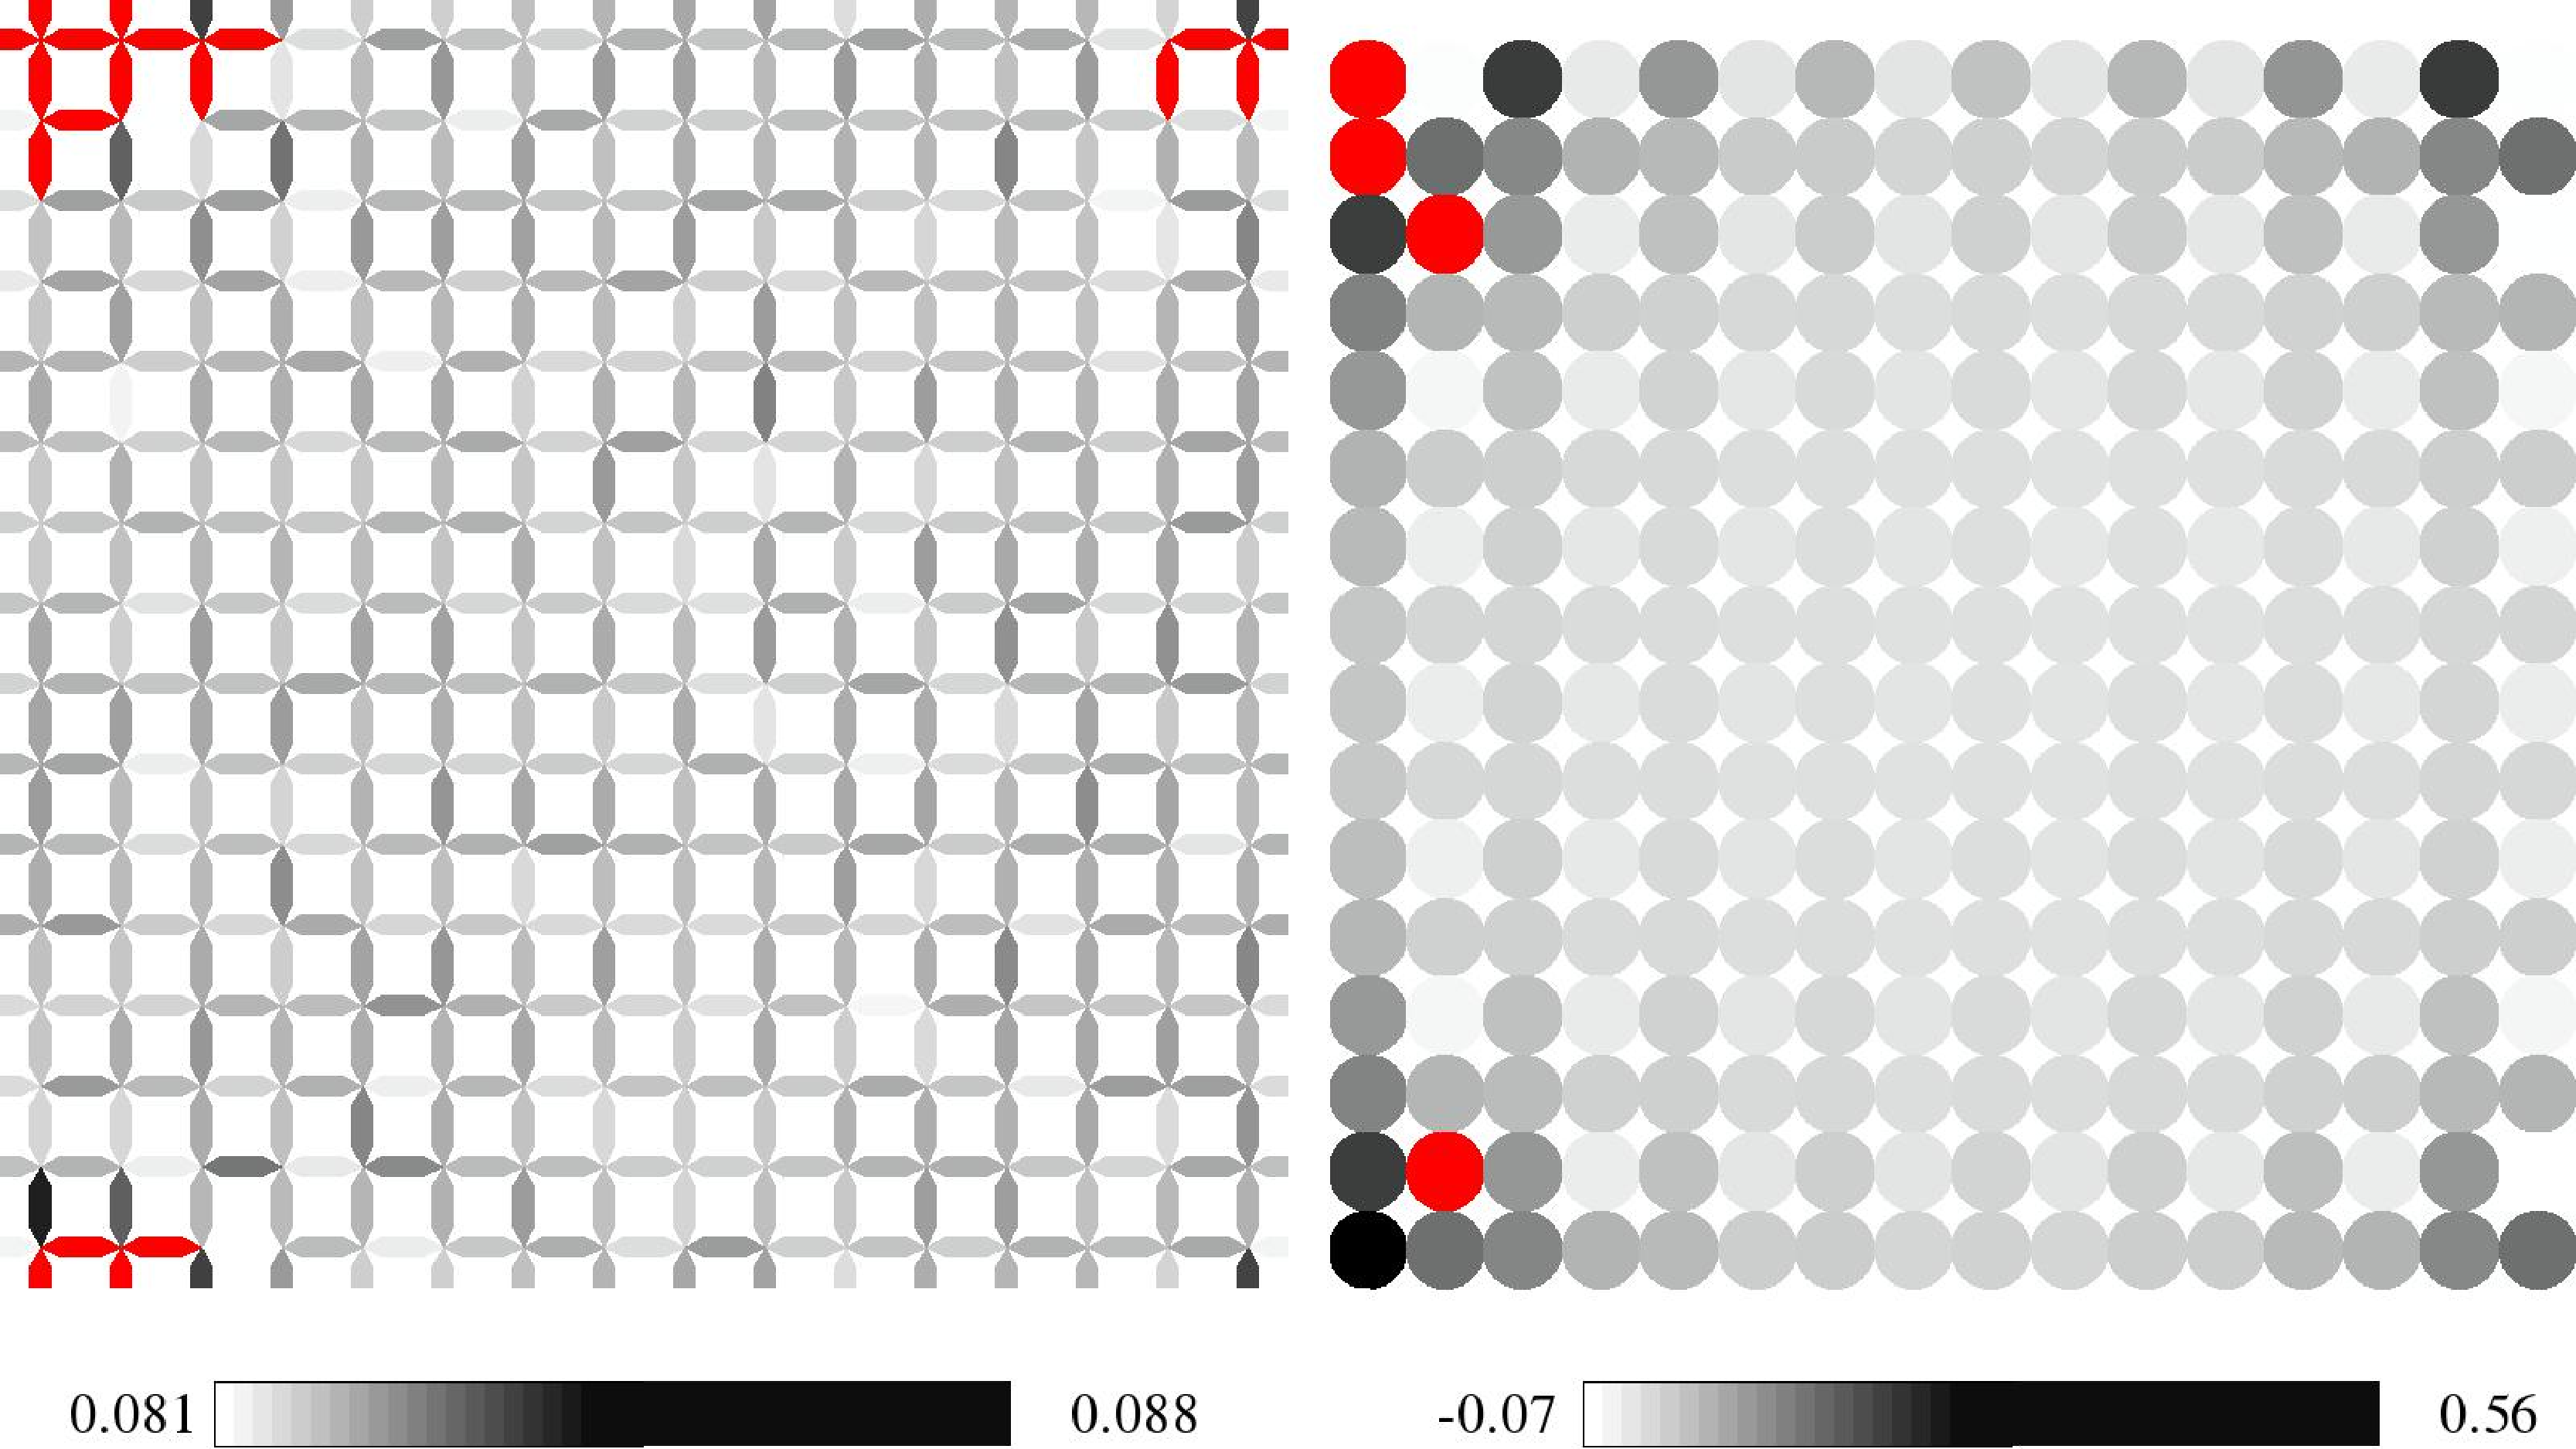
\includegraphics[width=0.8\linewidth]{dimer_gry_scale_qdpm.pdf}
        \caption{Gray scale (actualy data) of the dimer corelation between the dimer in the upper
        left corner and other dimers on a $16\times16$ lattice.}
        \label{fig:dimer_gry_scale_qdpm}
    \end{figure}

    \subsection{Correlation functions}

    \begin{equation}
        C_{\mathrm{dimer}} = \langle d_0 d_r \rangle - \langle d_0 \rangle   \langle d_r \rangle   
    \end{equation}

    \begin{figure}[htpb]
        \centering
        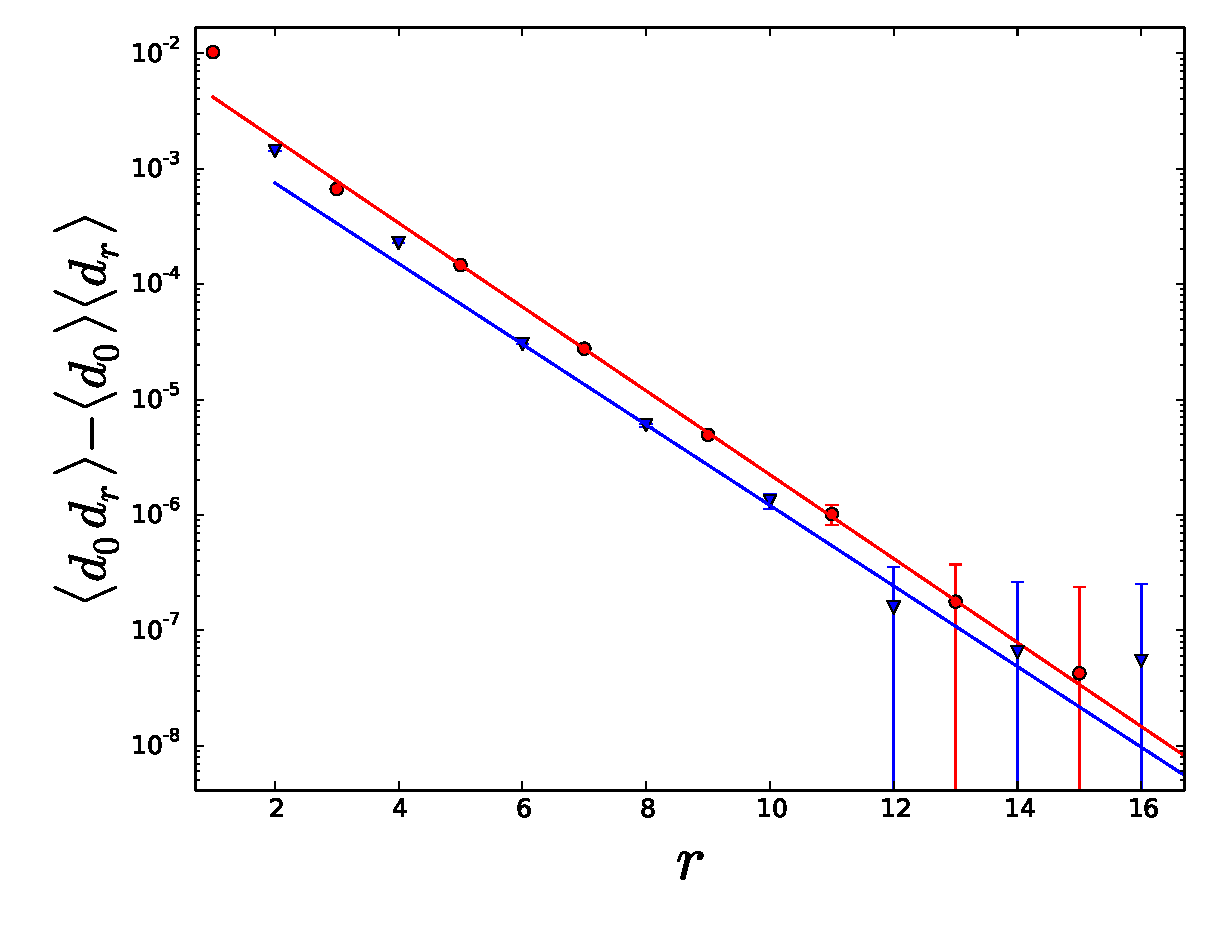
\includegraphics[width=0.8\linewidth]{spacial_dmr_cor.pdf}
        \caption{(Note: This figure was made using equal probabilities of plaquette flips and
        pentamer moves) Spacial correlation function of parallel dimers for the two different
        sublattices distinguished by their color (red, green).}
        \label{fig:spacial_dmr_cor}
    \end{figure}

    \subsection{Comparison to other models}

%%%%%%%%%%%%%%%%%%%%%%%%%%%%%%%%%%%%%%%%%%%%%%%%%%%%%%%%%%%%%%%%%%%%%%%%%%%%%%%%%%%%%%%%%%%%%%%
%%%%%%%%%%%%%%%%%%%%%%%%%%%%%%%%%%%%%%%%%%%%%%%%%%%%%%%%%%%%%%%%%%%%%%%%%%%%%%%%%%%%%%%%%%%%%%%
\section{Estimating the Gap}

%    \begin{table*}[htpb]
%    \setlength\tabcolsep{0.3cm}
%        \centering
%        \caption{$\Delta \tau = 150$}
%        \label{tab:label}
%        \begin{tabular}{l l l l l}
%            \hline\hline
%         L            		& 8x8                               		& 12x12                            		& 16x16					& 18x18 \\ 
%            \hline                                                                                                                           
%         frac 1.0     	&                                       		&                                  		&                                    		&  \\
%            \hline                                                                                                                           
%         Dimer        	&  $ 3(1) \times 10^{-2}$        	& $ 1.43(3) \times 10^{-2}$	& $0.81(2)\times 10^{-2}$  	& \\
%         $Z_2$ origin 	&  $ 0.787?(5)\times 10^{-2} $ 	& $ 0.344? (1)\times 10^{-2}$ 	& $0.198? (4)\times 10^{-2} $ 	&  \\
%         $Z_3$ origin 	&  NA                                   	& NA                               		& NA                                  	& \\
%            \hline                                                                                                                         
%         frac 0.9     	&                                       		&                                  		&                                     		&  \\
%            \hline                                                                                                                          
%         Dimer origin 	&  $ 0.419(1)\times 10^{-2} $    	& $ 0.406(2)\times 10^{-2} $ 	& $0.429(1)\times 10^{-2} $   	&  $ 0.405(2)\times 10^{-2} $\\
%         $Z_2$ origin 	&  $ 0.216?(2)\times 10^{-2} $ 	& $ 0.141?(1)\times 10^{-2} $ 	& $0.129?(2)\times 10^{-2} $	&  $ 0.126?(2)\times 10^{-2} $\\
%         $Z_3$ origin 	&  $ 0.346?(4)\times 10^{-2} $ 	& $ 0.348(1)\times 10^{-2} $ 	& $0.359?(4)\times 10^{-2} $	&  $ 0.355?(3)\times 10^{-2}$\\
%            \hline                                                                                                                          
%         frac 0.5     	&                                       		&                                   		&                                    		& \\
%            \hline                                                                                                                          
%         Dimer origin 	&                                       		& $ 2.075(9)\times 10^{-2} $ 	& $2.05(1) \times 10^{-2}$		&  $ $ \\
%         $Z_2$ origin 	&                                       		& $ 0.615?(2)\times 10^{-2} $ 	& $0.614?(3)\times 10^{-2} $	&  $ $ \\
%         $Z_3$ origin 	&                                       		& $ 1.939(2)\times 10^{-2} $ 	& $1.927(2)\times 10^{-2} $	&  $ $  
%        \end{tabular}
%    \end{table*}

    \begin{table*}[htpb]
    \setlength\tabcolsep{0.3cm}
        \centering
        \caption{$\Delta \tau = 150$}
        \label{tab:label}
        \begin{tabular}{l l l l}
            \hline\hline
                        & Dimer                 & $Z_2$ double ($L/2$)  &  $Z_3$ single (origin)     \\   
            \hline
            frac 1.0    &  &  & \\
            $8\times8$  & $3.(3)\times10^{-2}$  &                       &                            \\
            $12\times12$& $1.4(5)\times10^{-2}$ &                       &                            \\
            $16\times16$&                       &                       &                            \\
            $18\times18$&                       &                       &                            \\
            \hline
            frac 0.9    &  &  & \\
            $8\times8$  & $0.35(5)\times10^{-2}$&$0.102(1)\times10^{-2}$& $0.306(3)\times10^{-2}$     \\
            $12\times12$& $0.35(7)\times10^{-2}$&$0.25(5)\times10^{-2}$ & $0.316(4)\times10^{-2}$    \\
            $16\times16$& $0.35(7)\times10^{-2}$&$0.36(3)\times10^{-2}$ & $0.316(8)\times10^{-2}$    \\
            $18\times18$&                       &                       &                            \\
            \hline
            frac 0.5    &  &  & \\
            $8\times8$  & $1.0(6)\times10^{-2}$ &$0.05(5)\times10^{-2}$ & $1.7(1)\times10^{-2}$     \\
            $12\times12$& $1.5(7)\times10^{-2}$ &                       & $1.9(7)\times10^{-2}$      \\
            $16\times16$&                       &                       &                            \\
            $18\times18$&                       &                       &                            \\
        \end{tabular}
    \end{table*}


    \subsection{Imaginary time vison correlations}
    \begin{figure}[htpb]
        \centering
        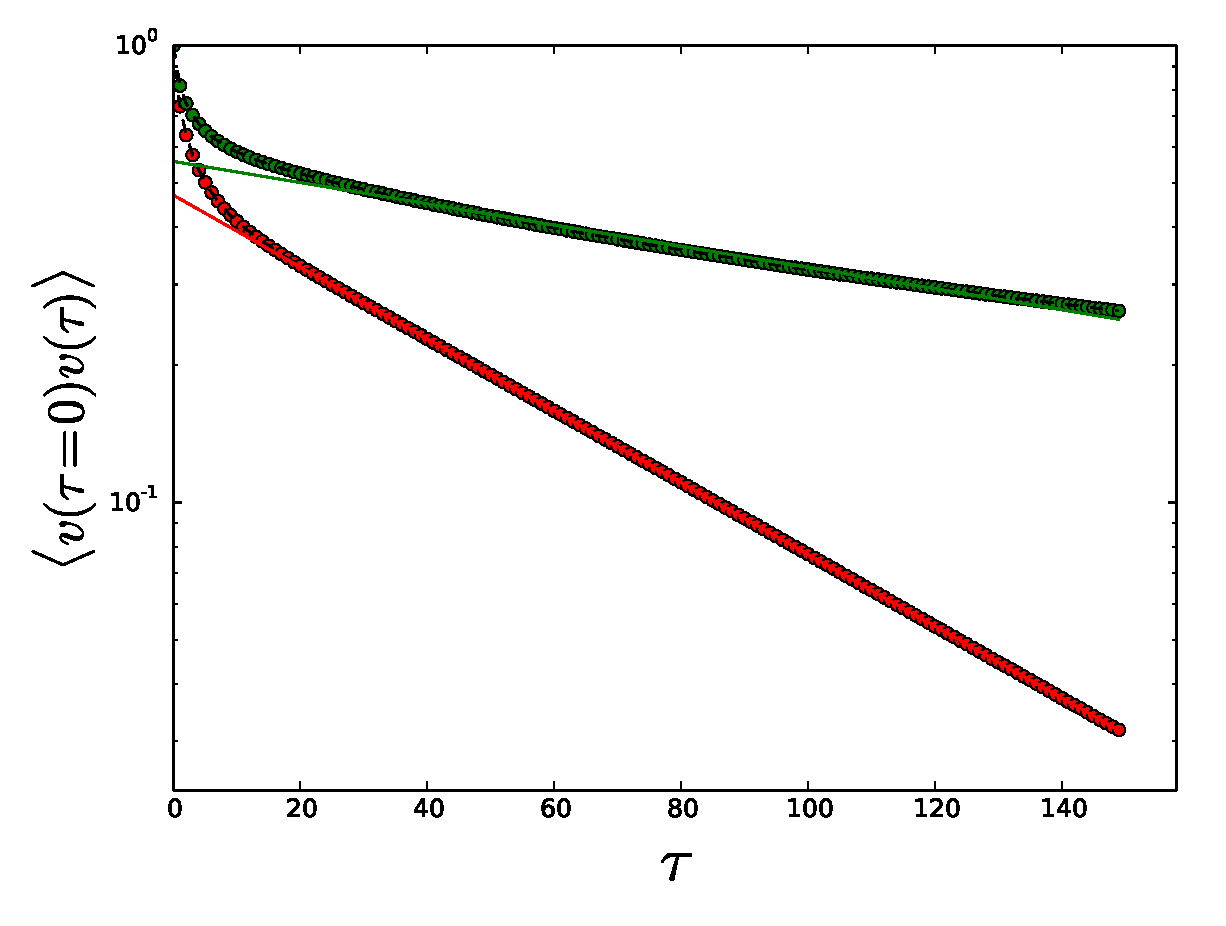
\includegraphics[width=0.8\linewidth]{z2_origin_vison_time_cor.pdf}
        \caption{Imaginary time $z_2$ \textit{single} vison correlations at the origin in the QDM model (red) and QDPM
        model (green) on an $8\times8$ lattice. For the QDPM the dimer/pentamer move fraction is $0.9$.}
        \label{fig:name}
    \end{figure}

    \subsection{Imaginary time dimer correlations}
    \begin{figure}[htpb]
        \centering
        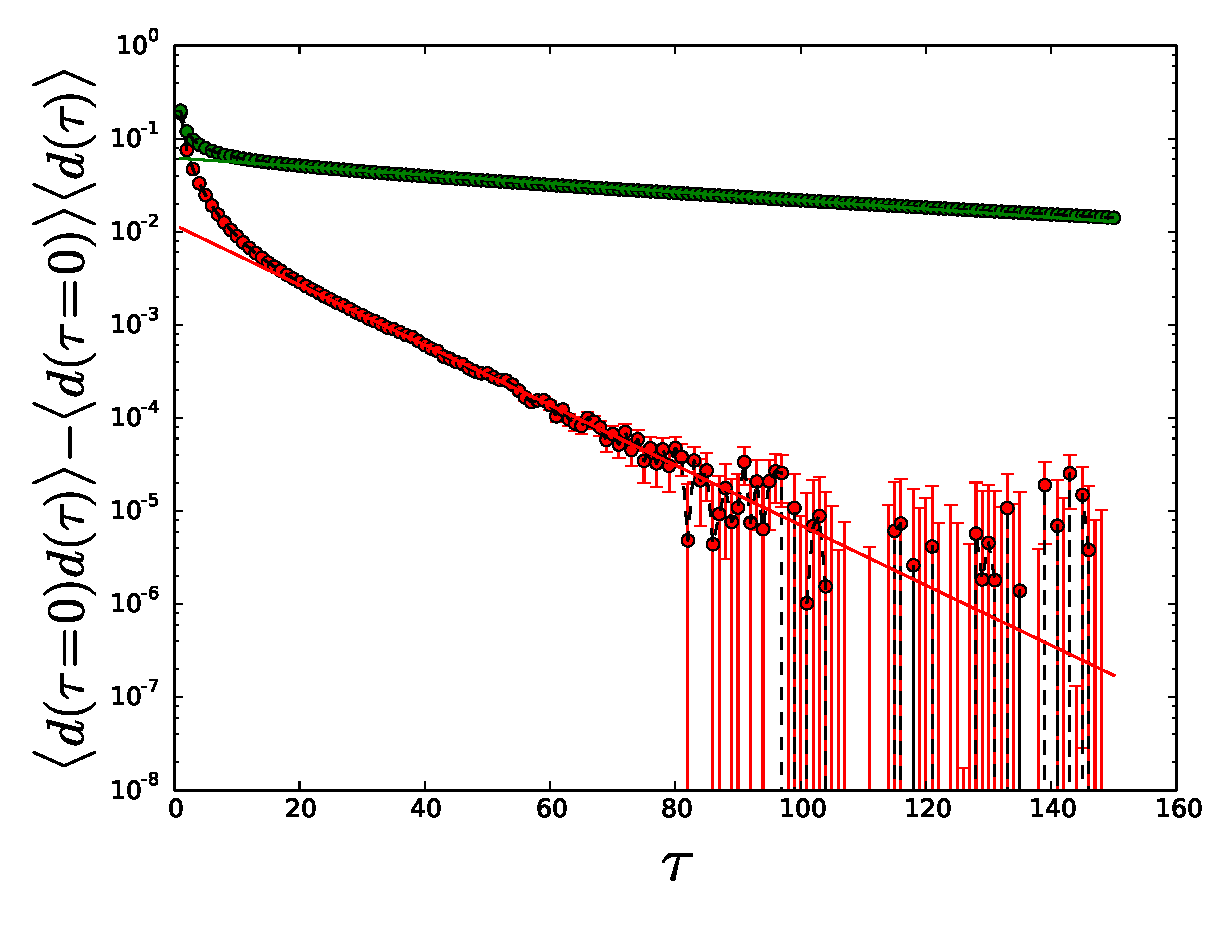
\includegraphics[width=0.8\linewidth]{dimer_origin_time_cor.pdf}
        \caption{Imaginary time dimer correlations of a single dimer in the QDM model (red) and QDPM
        model (green) on an $8\times8$ lattice. For the QDPM the dimer/pentamer move fraction is $0.9$. }
        \label{fig:}

    \end{figure}

%%%%%%%%%%%%%%%%%%%%%%%%%%%%%%%%%%%%%%%%%%%%%%%%%%%%%%%%%%%%%%%%%%%%%%%%%%%%%%%%%%%%%%%%%%%%%%%
%%%%%%%%%%%%%%%%%%%%%%%%%%%%%%%%%%%%%%%%%%%%%%%%%%%%%%%%%%%%%%%%%%%%%%%%%%%%%%%%%%%%%%%%%%%%%%%
\section{Discussion}

\bibliographystyle{apsrev4-1}
\bibliography{QDPM}

\end{document}
